\documentclass{ppgeesa}

\usepackage[hidelinks]{hyperref}

\usepackage{wrapfig}
\usepackage{graphicx}
\usepackage{epstopdf}
\usepackage{animate}
\graphicspath{{../fig/}}

\usepackage{amsmath}
\usepackage{amssymb}
\usepackage{amsfonts}
\usepackage{amsthm}
\usepackage{mathtools}
\usepackage{bm}
\usepackage{esvect}
\usepackage{resizegather}
\mathtoolsset{showonlyrefs}

\DeclareMathOperator{\trace}{tr}
\DeclareMathOperator{\rank}{\rho}
\newcommand*{\Round}[1]{\left(#1\right)}
\newcommand*{\Curly}[1]{\left\{#1\right\}}
\newcommand*{\Set}[1]{\Curly{#1}}
\newcommand*{\Prod}{\,}
\newcommand*{\Bold}[1]{\boldsymbol{\mathbf{#1}}}
\newcommand*{\Matr}[1]{\Bold{#1}}
\newcommand*{\Vect}[1]{\vv{\Bold{#1}}}
\newcommand*{\Inv}[1]{{#1}^{-1}}
\newcommand*{\Transp}[1]{{#1}^{T}}
\newcommand*{\Trace}[1]{\trace\Round{#1}}
\newcommand*{\Rank}[1]{\rank\Round{#1}}
\newcommand*{\ForAll}{\:\:\forall\,}
\newcommand*{\Viff}{\\\Updownarrow\\}
\newcommand*{\Vimplies}{\\\Downarrow\\}

\usepackage{siunitx}
\sisetup{output-decimal-marker = {,}}
\sisetup{exponent-product = {\cdot}}

\usepackage{pgffor}
\usepackage[section]{placeins}

\hyphenation{MATLAB}

\begin{document}
\bstctlcite{IEEEBST:Brazilian}

\title{Estimativa da Região de Atração de Sistema Não-Linear na Representação Diferencial-Algébrica por Inequações Matriciais Lineares}
\author{Guilherme de Paoli Beal
  \\
  {\small Universidade Federal do Rio Grande do Sul}
  \thanks{G. Beal, guilherme.beal@ufrgs.br}
}
\maketitle
\thispagestyle{empty}\pagestyle{empty}

\begin{abstract}
  Este trabalho demonstra a aplicação de inequações matriciais lineares para a obtenção de uma estimativa da região de atração da origem para um sistema não-linear em sua representação diferencial-algébrica.
  O procedimento é exemplificado pela aplicação em sistemas não-lineares bidimensionais.
\end{abstract}

\begin{IEEEkeywords}
  Sistema Não-Linear,
  Região de Atração da Origem,
  Representação Diferencial-Algébrica,
  Inequações Matriciais Lineares
\end{IEEEkeywords}

\section{Introdução}
A região de atração de um sistema é definida como o espaço de condições iniciais que convergem para um determinado ponto de equilíbrio estável.
Tipicamente, este ponto é considerado a origem do sistema, sem perda de generalidade \cite{book:Khalil2002}.

A determinação da região de atração da origem de sistemas não-lineares é de grande interesse.
Fisicamente, essa região é considerada um espaço seguro de operação.
No entanto, a determinação analítica da região de atração é, em geral, difícil ou até impossível \cite{book:Khalil2002}.
Assim, a estimação desta região é de grande valor.

Um dos métodos tipicamente empregados para estimação da região de atração de origem faz uso do conceito de estabilidade de Lyapunov.
Se existe uma função de Lyapunov válida em um determinado domínio, e existe uma curva de nível desta função no interior deste domínio, então a região no interior desta curva de nível é uma estimativa da região de atração da origem.
No entanto, a depender da função de Lyapunov, essa estimativa pode ser conservador, isto é, consideravelmente menor do que a verdadeira região de atração.

Uma maneira de obter estimativas menos conservadoras é a otimização numérica de algum critério.
Se o problema puder ser expresso por um conjunto de equações convexas, então a otmimização pode ser realizada por Inequações Matriciais Lineares --- em inglês, \textit{Linear Matrix Inequalities} (LMIs).
Uma maneira de adequar sistemas não-lineares para essa abordagem é transformando-os para uma representação diferencial-algébrica --- em inglês, \textit{Differential-Algebraic Representation} (DAR).

Com base na formulação em \cite{article:Coutinho2010}, o presente trabalho apresenta a obtenção de um conjunto de LMIs para sistemas não-lineares autônomos e não-forçados, transformados em DAR, a partir de uma função de Lyapunov quadrática.
O método é exemplificado pela aplicação em dois sistemas bidimensionais.
A implementação das LMIs foi realizada em MATLAB utilizando o pacote YALMIP \cite{proceedings:Lofberg2004}, e o código desenvolvido está disponível em \href{https://github.com/GuiBeal/RoA-LMI-DAR}{github.com/GuiBeal/RoA-LMI-DAR}.

\section{Definição do Problema}
Seja um sistema não-linear autônomo e não-forçado representado por
\begin{equation}\label{eq:system}
  \dot{\Vect{x}} = \Vect{f}(\Vect{x})
  ,
\end{equation}
em que $\Vect{x} \in \mathcal{B}_x$ é o vetor de estados, $\mathcal{B}_x \subset \mathbb{R}^n$ é uma região politópica (que será definida posteriormente) e $\Vect{f} \colon \mathbb{R}^n \to \mathbb{R}^n$ é uma função vetorial racional ou polinomial em $\Vect{x}$ que representa a dinâmica do sistema.
Assume-se que $\Vect{f}$ é localmente Lipschitz.
Assume-se, ainda, que a origem $\Vect{0} \in \mathcal{B}_x$ é um ponto de equilíbrio, isto é,
\begin{equation}
  \Vect{f}(\Vect{0}) = \Vect{0}
  .
\end{equation}

A região de atração da origem $\mathcal{R} \subset \mathbb{R}^n$ é o conjunto de todas as condições iniciais $\Vect{x}(0)$ a partir das quais a resposta do sistema tende à origem, expresso por
\begin{equation}
  \Vect{x}(0) \in \mathcal{R}
  \implies
  \lim_{t \to \infty} \Vect{x}(t) = \Vect{0}
  .
\end{equation}

\section{Conceitos Preliminares}

\subsection{Representação Diferencial-Algébrica}
O sistema em \eqref{eq:system} pode ser representado em formato algébrico-diferencial como
\begin{equation}
  \left\{\begin{aligned}
    \dot{\Vect{x}} &= \Matr{A}_1(\Vect{x}) \Prod \Vect{x} + \Matr{A}_2(\Vect{x}) \Prod \Vect{z}(\Vect{x})
    \\
    \Vect{0} &= \Matr{\Omega}_1(\Vect{x}) \Prod \Vect{x} + \Matr{\Omega}_2(\Vect{x}) \Prod \Vect{z}(\Vect{x})
  \end{aligned}\right.
  .
\end{equation}
Nesta representação, $\Vect{z} \colon \mathbb{R}^n \to \mathbb{R}^{n_z}$ é uma função vetorial contendo termos racionais e polinomiais (de ordem 2 ou maior) em $\Vect{x}$ presentes em $\Vect{f}$.
Além disso, $\Matr{A}_1 \colon \mathbb{R}^n \to \mathbb{R}^{n \times n}$, $\Matr{A}_2 \colon \mathbb{R}^n \to \mathbb{R}^{n \times n_z}$, $\Matr{\Omega}_1 \colon \mathbb{R}^n \to \mathbb{R}^{n_z \times n}$ e $\Matr{\Omega}_2 \colon \mathbb{R}^n \to \mathbb{R}^{n_z \times n_z}$ são funções matriciais afins em $\Vect{x}$.

Para que a representação seja bem definida, é necessário que $\Matr{\Omega}_2$ tenha posto completo, isto é,
\begin{equation}
  \Rank{\Matr{\Omega}_2(\Vect{x})} = n_z \ForAll \Vect{x} \in \mathcal{B}_x
  .
\end{equation}
Com isso, as variáveis são relacionadas por
\begin{equation}
  \Vect{z}(\Vect{x}) = -\Inv{\Matr{\Omega}_2(\Vect{x})} \Prod \Matr{\Omega}_1(\Vect{x}) \Prod \Vect{x}
  \ForAll \Vect{x} \in \mathcal{B}_x
  .
\end{equation}

Todos os sistemas com função dinâmica $\Vect{f}$ racional podem ser transformados para DAR \cite{article:Coutinho2010}.
Destaca-se, porém, que a representação de um sistema não é única.

\subsection{Função de Lyapunov}
Seja uma função $V \colon \mathcal{B}_x \to \mathbb{R}$ continuamente diferenciável. Se existirem constantes $\varepsilon_1 \in \mathbb{R}^+$, $\varepsilon_2 \in \mathbb{R}^+$ e $\varepsilon_3 \in \mathbb{R}^+$ e as condições
\begin{equation}\label{eq:Lyapunov}
  \varepsilon_1 \Prod \Transp{\Vect{x}} \Prod \Vect{x} \leq V(\Vect{x}) \leq \varepsilon_2 \Prod \Transp{\Vect{x}} \Prod \Vect{x}
  \ForAll \Vect{x} \in \mathcal{B}_x
\end{equation}
e
\begin{equation}\label{eq:Lyapunov-diff}
  \dot{V}(\Vect{x}) \leq -\varepsilon_3 \Prod \Transp{\Vect{x}} \Prod \Vect{x}
  \ForAll \Vect{x} \in \mathcal{B}_x
  .
\end{equation}
forem satisfeitas, então $V$ é denominada função de Lyapunov e a origem é um ponto de equilíbrio assintoticamente estável.
Além disso,
\begin{equation}\label{eq:attraction-estimate}
  \hat{\mathcal{R}} = \left\{\Vect{x} \in \mathcal{B}_x \colon V(\Vect{x}) \leq 1\right\}
\end{equation}
é uma estimativa da região de atração da origem \cite{book:Khalil2002,article:Coutinho2010}.

Este trabalho limita-se a funções de Lyapunov quadráticas, definidas como
\begin{equation}\label{eq:Lyapunov-quadratic}
  V(\Vect{x})= \Transp{\Vect{x}} \Prod \Matr{P} \Prod \Vect{x}
  ,
\end{equation}
em que $\Matr{P} \in \mathbb{R}^{n \times n} \colon \Transp{\Matr{P}} = \Matr{P} > 0$ é uma matriz simétrica positiva definida.
A partir disso, tem-se que
\begin{equation}\label{eq:Lyapunov-quadratic-diff}
  \dot{V}(\Vect{x}) = \Transp{\dot{\Vect{x}}} \Prod \Matr{P} \Prod \Vect{x} + \Transp{\Vect{x}} \Prod \Matr{P} \Prod \dot{\Vect{x}}.
\end{equation}
Ademais, com essa função, $\hat{\mathcal{R}}$ é uma região elipsoidal.

% \subsubsection{Representação Estendida}
Utilizando o vetor estendido
\begin{equation}\label{eq:zeta}
  \Vect{\zeta}(\Vect{x}) = \begin{bmatrix} \Vect{x} \\ \dot{\Vect{x}} \\ \Vect{z}(\Vect{x}) \end{bmatrix}
\end{equation}
e as matrizes
\begin{equation}
  \Matr{\Sigma}(\Matr{P}) = \begin{bmatrix}
    \Matr{P}  & \Matr{0}   & \Matr{0}       \\
    \Matr{0}  & \Matr{0}_n & \Matr{0}       \\
    \Matr{0}  & \Matr{0}   & \Matr{0}_{n_z} \\
  \end{bmatrix}
\end{equation}
e
\begin{equation}
  \Matr{\Lambda}(\Matr{P}) = \begin{bmatrix}
    \Matr{0}_n & \Matr{P}   & \Matr{0}       \\
    \Matr{P}   & \Matr{0}_n & \Matr{0}       \\
    \Matr{0}   & \Matr{0}   & \Matr{0}_{n_z} \\
  \end{bmatrix}
  ,
\end{equation}
\eqref{eq:Lyapunov-quadratic} e \eqref{eq:Lyapunov-quadratic-diff} são reescritas como
\begin{equation}\label{eq:Lyapunov-extended}
  V(\Vect{x}) = \Transp{\Vect{\zeta}(\Vect{x})} \Prod \Matr{\Sigma}(\Matr{P}) \Prod \Vect{\zeta}(\Vect{x})
\end{equation}
e
\begin{equation}\label{eq:Lyapunov-diff-extended}
  \dot{V}(\Vect{x}) = \Transp{\Vect{\zeta}(\Vect{x})} \Prod \Matr{\Lambda}(\Matr{P}) \Prod \Vect{\zeta}(\Vect{x})
  .
\end{equation}
Além disso,
\begin{equation}
  \Matr{\mathcal{M}}(\Vect{x}) = \begin{bmatrix}
    \Matr{A}_1(\Vect{x})      & -\Matr{I}_n & \Matr{A}_2(\Vect{x})      \\
    \Matr{\Omega}_1(\Vect{x}) & \Matr{0}    & \Matr{\Omega}_2(\Vect{x}) \\
  \end{bmatrix}
\end{equation}
estabelece uma relação entre as variáveis através de
\begin{equation}\label{eq:M-zeta}
  \Matr{\mathcal{M}}(\Vect{x}) \Prod \Vect{\zeta}(\Vect{x}) = \vec{0}
  .
\end{equation}
Esse formato será essencial para a obteção das LMIs.

\subsection{Politopo}
O politopo $\mathcal{B}_x$ é delimitado por suas $n_e$ faces $\Vect{h}_k$, isto é,
\begin{equation}\label{eq:polytope}
  \mathcal{B}_x
  = \Set{\Vect{x} \in \mathbb{R}^n \colon \Transp{\Vect{h}_k} \Prod \Vect{x} \leq 1 \,,\; k = 1, \dotsc, n_e}
  .
\end{equation}
O politopo pode, ainda, ser representado por seu conjunto de vértices $\mathcal{V}(\mathcal{B}_x)$.

% \subsubsection{Representação Estendida}
Utilizando novamente o vetor estendido em \eqref{eq:zeta} e estendendo as faces como
\begin{equation}
  \Vect{\vartheta}\Round{\Vect{h}_k} = \begin{bmatrix} \Vect{h}_k \\ \Vect{0}_n \\ \Vect{0}_{n_z} \end{bmatrix}
  ,
\end{equation}
\eqref{eq:polytope} é reescrita como
\begin{equation}\label{eq:polytope-extended}
  \begin{aligned}
    \mathcal{B}_x
    &= \Set{\Vect{x} \in \mathbb{R}^n \colon \Transp{\Vect{\vartheta}\Round{\Vect{h}_k}} \Prod \Vect{\zeta}(\Vect{x}) \leq 1 \,,\; k = 1, \dotsc, n_e}
    .
  \end{aligned}
\end{equation}
Esse formato será útil para a obtenção de $\hat{\mathcal{R}}$.

\subsection{Estimativa da Região de Atração da Origem}
A região de atração da origem deve estar no interior do politopo, ou seja, $\hat{\mathcal{R}} \subset \mathcal{B}_x$.
Utilizando \eqref{eq:Lyapunov-extended} e \eqref{eq:polytope-extended}, essa condição é expressa por
\begin{equation}
  \Transp{\Vect{\vartheta}(\Vect{h}_k)} \Prod \Vect{\zeta}(\Vect{x}) \leq 1
  \ForAll \Vect{x} \in \mathbb{R}^n \colon \Transp{\Vect{\zeta}(\Vect{x})} \Prod \Matr{\Sigma}(\Matr{P}) \Prod \Vect{\zeta}(\Vect{x}) \leq 1
  \,,\\ k = 1, \dotsc, n_e
  ,
\end{equation}
ou, ainda,
\begin{equation}\label{eq:region-attraction-pre-S}
  \begin{gathered}
    2 \Prod \Transp{\Vect{\vartheta}(\Vect{h}_k)} \Prod \Vect{\zeta}(\Vect{x}) - 2 \leq 0
    \ForAll \Vect{x} \colon \Transp{\Vect{\zeta}(\Vect{x})} \Prod \Matr{\Sigma}(\Matr{P}) \Prod \Vect{\zeta}(\Vect{x}) -1 \leq 0
    \,,\\ k = 1, \dotsc, n_e
    .
  \end{gathered}
\end{equation}

Definindo o vetor
\begin{equation}
  \Vect{\varsigma}(\Vect{x}) = \begin{bmatrix} \Vect{\zeta}(\Vect{x}) \\ 1 \end{bmatrix}
\end{equation}
e aplicando \textit{S-Procedure} \cite{book:Boyd2004} em \eqref{eq:region-attraction-pre-S}, obtém-se
\begin{equation}\label{eq:region-attraction-post-S}
  \begin{gathered}
    \Transp{\Vect{\varsigma}(\Vect{x})} \Prod \left(\begin{bmatrix}
      \Matr{\Sigma}(\Matr{P}) & \Vect{0} \\
      \Transp{\Vect{0}}       & -1       \\
    \end{bmatrix} - \nu \Prod \begin{bmatrix}
      \Matr{0}                              & \Vect{\vartheta}(\Vect{h}_k) \\
      \Transp{\Vect{\vartheta}(\Vect{h}_k)} & -2                           \\
    \end{bmatrix}\right) \Prod \Vect{\varsigma}(\Vect{x}) \geq 0
    \,,\\ k = 1, \dotsc, n_e
    ,
  \end{gathered}
\end{equation}
\vspace{-5pt}
em que $\nu \in \mathbb{R}^+$ é uma constante livre.
Definindo a matriz
\begin{equation}
  \Matr{\Pi}(\Matr{P}, \Vect{h}_k, \nu) = \begin{bmatrix}
    \Matr{\Sigma}(\Matr{P})                          & -\nu \Prod \Vect{\vartheta}(\Vect{h}_k) \\
    -\nu \Prod \Transp{\Vect{\vartheta}(\Vect{h}_k)} & 2 \Prod \nu - 1                         \\
  \end{bmatrix}
  ,
\end{equation}
\eqref{eq:region-attraction-post-S} é reescrita como
\begin{equation}\label{eq:sigma-Pi}
  \Transp{\Vect{\varsigma}(\Vect{x})} \Prod \Matr{\Pi}(\Matr{P}, \Vect{h}_k, \nu) \Prod \Vect{\varsigma}(\Vect{x}) \geq 0
  \,,\; k = 1, \dotsc, n_e
  .
\end{equation}
Finalmente,
\begin{equation}
  \Matr{\mathcal{N}}(\Vect{x}) = \begin{bmatrix}
    \Matr{A}_1(\Vect{x})      & -\Matr{I}_n & \Matr{A}_2(\Vect{x})      & \Vect{0} \\
    \Matr{\Omega}_1(\Vect{x}) & \Matr{0}    & \Matr{\Omega}_2(\Vect{x}) & \Vect{0} \\
    -\Matr{I}_n               & \Matr{0}    & \Matr{0}                  & \Vect{x} \\
  \end{bmatrix}
\end{equation}
estabelece uma relação entre as variáveis através de
\begin{equation}\label{eq:N-sigma}
  \Matr{\mathcal{N}}(\Vect{x}) \Prod \Vect{\varsigma}(\Vect{x}) = \Vect{0}
  .
\end{equation}
A partir desse formato serão obtidas as LMIs.

\section{Inequações Matriciais Lineares}
A seguir enunciam-se as LMIs que garantem as condições da função de Lyapunov, bem como que $\hat{\mathcal{R}} \subset \mathcal{B}_x$.
Com a matriz $\Matr{P}$ resultante, $\hat{\mathcal{R}}$ é obtida conforme \eqref{eq:attraction-estimate}.

Por definição, tem-se que
\begin{gather}
  \label{eq:constraint-P}
  \Matr{P} = \Transp{\Matr{P}} > 0
  ,
  \\
  \label{eq:constraint-nu}
  \nu > 0
  .
\end{gather}
Pela aplicação do Lema de Finsler \cite{proceedings:Oliveira2001} obtém-se a seguir um conjunto de inequações.
Como as matrizes são funções afins de $\Vect{x}$, a validade das mesmas em toda o politopo $\mathcal{B}_x$ pode ser testada avaliando as inequações em seus vértices $\mathcal{V}(\mathcal{B}_x)$
A partir de \eqref{eq:Lyapunov-extended} e \eqref{eq:M-zeta}, obtém-se
\begin{equation}\label{eq:constraint-sigma}
  \begin{aligned}
    \Matr{\Sigma}(\Matr{P}) + \Matr{L} \Prod \Matr{\mathcal{M}}(\Vect{x}) + \Transp{\Matr{\mathcal{M}}(\Vect{x})} \Prod \Transp{\Matr{L}} &> 0
    \ForAll \Vect{x} \in \mathcal{V}(\mathcal{B}_x)
    ,
    % \\\vphantom{\sum} % Fix eq numbering
  \end{aligned}
\end{equation}
em que $\Matr{L} \in \mathbb{R}^{(2 \Prod n + n_z) \times (n + n_z)}$ é uma matriz livre.
Por sua vez, \eqref{eq:Lyapunov-diff-extended} e \eqref{eq:M-zeta} fornecem
\begin{equation}\label{eq:constraint-lambda}
  \begin{aligned}
    -\Matr{\Lambda}(\Matr{P}) + \Matr{W} \Prod \Matr{\mathcal{M}}(\Vect{x}) + \Transp{\Matr{\mathcal{M}}(\Vect{x})} \Prod \Transp{\Matr{W}} &> 0
    \ForAll \Vect{x} \in \mathcal{V}(\mathcal{B}_x)
    ,
  \end{aligned}
\end{equation}
em que $\Matr{W} \in \mathbb{R}^{(2 \Prod n + n_z) \times (n + n_z)}$ é uma matriz livre.
Finalmente, a partir de \eqref{eq:sigma-Pi} e \eqref{eq:N-sigma}, tem-se
\begin{equation}\label{eq:constraint-pi}
  \begin{gathered}
    \Matr{\Pi}(\Matr{P}, \Vect{h}_k, \nu) + \Matr{R}_k \Prod \Matr{\mathcal{N}}(\Vect{x}) + \Transp{\Matr{\mathcal{N}}(\Vect{x})} \Prod \Transp{\Matr{R}_k} > 0
    \\\ForAll \Vect{x} \in \mathcal{V}(\mathcal{B}_x)
    \,,\; k = 1, \dotsc, n_e
    ,
  \end{gathered}
\end{equation}
em que $\Matr{R}_k \in \mathbb{R}^{(2 \Prod n + n_z + 1) \times (2 \Prod n + n_z)}$ são matrizes livres.

% \subsection{Otimização}
A formulação por LMIs permite maximizar a região $\hat{\mathcal{R}}$ através de algum critério.
Note que $\hat{\mathcal{R}}$ é dependente da matriz $\Matr{P}$, conforme \eqref{eq:attraction-estimate}, e é, portanto, elipsoidal.
Assim, a direção da elipse é associado aos autovetores de $\Matr{P}$, enquanto o tamanho em cada direção é relacionado ao autovalor associado.
Dentre os critérios de otimização, citam-se:
maximização do menor eixo;
maximização do volume;
maximização em alguma direção; e
minimização do traço.
Este último, expresso por
\begin{equation}\label{eq:objective}
  \min_{\Matr{P}} \Trace{\Matr{P}}
  ,
\end{equation}
é o critério empregado nos exemplos deste trabalho.

Por fim, é necessário arbitrar um politopo $\mathcal{B}_x$.
Por simplicidade, escolhe-se um politopo losangular, cujas arestas tem comprimento $a$.
O mesmo é definido por quatro faces:
\begin{equation}
  \begin{gathered}
    \Vect{h}_1 = \dfrac{1}{a} \Prod \begin{bmatrix} 1 \\ 1 \end{bmatrix}
    ,\;
    \Vect{h}_2 = \dfrac{1}{a} \Prod \begin{bmatrix} 1 \\ -1 \end{bmatrix}
    ,\;
    \Vect{h}_3 = \dfrac{1}{a} \Prod \begin{bmatrix} -1 \\ -1 \end{bmatrix}
    ,\;
    \Vect{h}_4 = \dfrac{1}{a} \Prod \begin{bmatrix} -1 \\ 1 \end{bmatrix}
    ,
  \end{gathered}
  \\
  n_e = 4
  .
\end{equation}
Ademais, seus vértices são
\begin{equation}\label{eq:vertex}
  \mathcal{V}(\mathcal{B}_x) = \Set{
    \begin{bmatrix} a \\ 0 \end{bmatrix}
    ,
    \begin{bmatrix} 0 \\ -a \end{bmatrix}
    ,
    \begin{bmatrix} -a \\ 0 \end{bmatrix}
    ,
    \begin{bmatrix} 0 \\ a \end{bmatrix}
  }
  .
\end{equation}

No entanto, o máximo politopo que garante \eqref{eq:Lyapunov} e \eqref{eq:Lyapunov-diff} é desconhecido.
A abordagem é, portanto, inicializá-lo pequeno e aumentá-lo gradativamente enquanto as LMIs forem factíveis.
No caso losangular, isso corresponde a incrementar $a$.

Sob as condições propostas, o problema de otimização por LMIs é assim sintetizado:
objetiva-se otimizar \eqref{eq:objective} sujeito às restrições \eqref{eq:constraint-P}, \eqref{eq:constraint-nu}, \eqref{eq:constraint-sigma}, \eqref{eq:constraint-lambda} e \eqref{eq:constraint-pi}.

\section{Exemplos}

A seguir apresentam-se exemplos de aplicação do método proposto.
Para permitir a visualização gráfica, os exemplos limitam-se a sistemas bidimensionais.

\subsection{Exemplo 1}
O sistema deste exemplo provém de \cite[Exemplo~8.6]{book:Khalil2002}.
Considere um sistema com a seguinte função dinâmica:
\begin{equation}
  \Vect{f}(\Vect{x})
  = \begin{bmatrix}
    x_2
    \\
    -x_1 -x_2 + \frac{1}{3} \Prod {x_1}^3
  \end{bmatrix}
\end{equation}
Para sua representação diferencial-algébrica, utiliza-se o vetor
\begin{gather}
  \Vect{z}(\Vect{x}) = \begin{bmatrix} {x_1}^2 \end{bmatrix}
  ,
  \\
  n_z = 1
  .
\end{gather}
Assim, a representação é obtida com
\begin{align}
  \Matr{A}_1(\Vect{x})
  &= \begin{bmatrix}
     0 &  1 \\
    -1 & -1 \\
  \end{bmatrix}
  ,&
  \Matr{A}_2(\Vect{x})
  &= \begin{bmatrix}
    0                     \\
    \frac{1}{3} \Prod x_1 \\
  \end{bmatrix}
  ,
  \\
  \Matr{\Omega}_1(\Vect{x})
  &= \begin{bmatrix}
    x_1 & 0 \\
  \end{bmatrix}
  ,&
  \Matr{\Omega}_2(\Vect{x})
  &= \begin{bmatrix}
    -1 \\
  \end{bmatrix}
  .
\end{align}

As variáveis livres nas LMIs e suas dimensões são
\begin{gather}
  \nu \in \mathbb{R} \colon \nu > 0
  ,\\
  \Matr{P} \in \mathbb{R}^{2 \times 2} \colon \Matr{P} = \Matr{P}^T > 0
  ,\\
  \Matr{L} \in \mathbb{R}^{5 \times 3}
  ,\\
  \Matr{W} \in \mathbb{R}^{5 \times 3}
  ,\\
  \Matr{R}_k \in \mathbb{R}^{6 \times 5}
  ,\; k = 1, 2, 3, 4
  .
\end{gather}
A aresta do politopo é inicializada como $a = \num{0.2}$ e incrementada em $\num{0.1}$ enquanto o problema de otimização é factível.
O máximo politopo é obtido com $a = \num{2.9}$.
A Figura \ref{fig:rao1} exibe o politopo, a estimativa da região de atração da origem e o campo vetorial de $\Vect{f}$.

\begin{figure}[h]
  \centering
  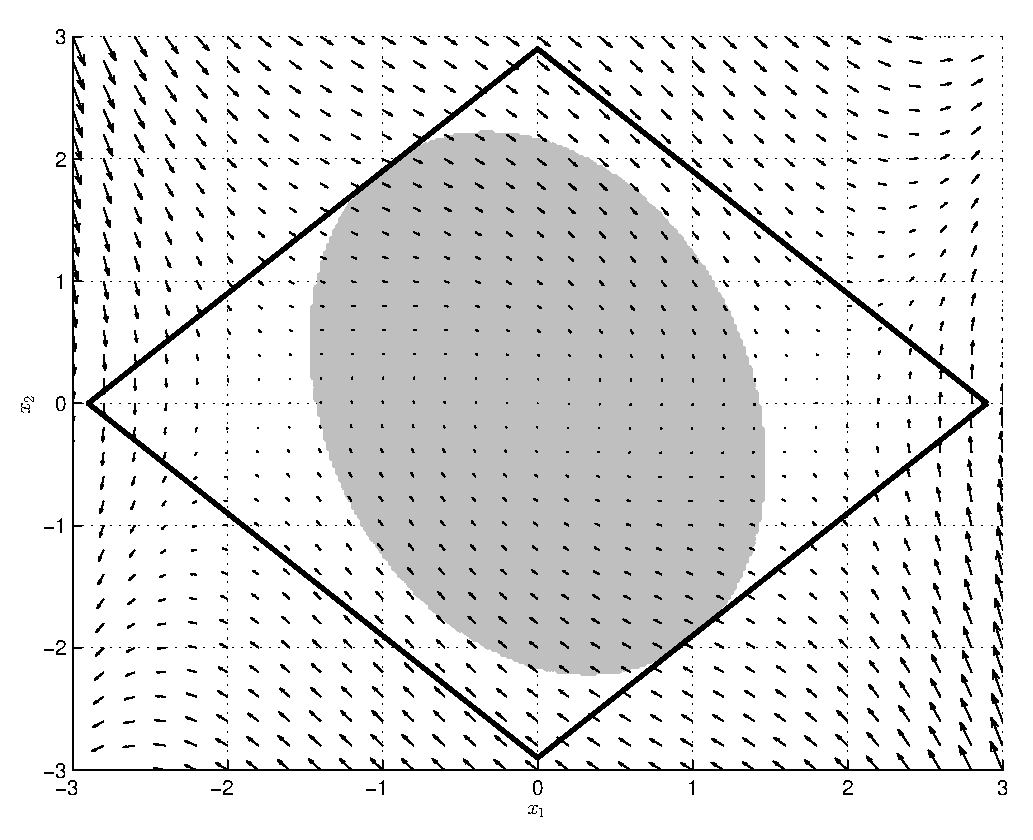
\includegraphics[width=0.95\linewidth]{exemplo1_28.eps}
  \caption{Estimativa da Região de Atração da Origem para o Exemplo 1.}
  \label{fig:rao1}
\end{figure}

\subsection{Exemplo 2}
Para este exemplo, considere um sistema com a seguinte função dinâmica:
\begin{equation}
  \begin{aligned}
    \Vect{f}(\Vect{x})
    &= \begin{bmatrix}
      -x_2
      \\
      x_1 -x_2 \Prod \Round{1 -{x_1}^2 + \num{0.1} \Prod {x_1}^4}
    \end{bmatrix}
    \\
    &= \begin{bmatrix}
      -x_2
      \\
      x_1 -x_2 -{x_1}^2 \Prod x_2 + \num{0.1} \Prod {x_1}^4 \Prod x_2
    \end{bmatrix}
    .
  \end{aligned}
\end{equation}
Para sua representação diferencial-algébrica, utiliza-se o vetor
\begin{gather}
  \Vect{z}(\Vect{x}) = \begin{bmatrix} {x_1}^2 \\ {x_1}^3 \\ {x_1}^4 \end{bmatrix}
  ,
  \\
  n_z = 3
  .
\end{gather}
Assim, a representação é obtida com
\begin{align}
  \Matr{A}_1(\Vect{x})
  &= \begin{bmatrix}
    0 & -1 \\
    1 & -1 \\
  \end{bmatrix}
  ,&
  \Matr{A}_2(\Vect{x})
  &= \begin{bmatrix}
    0    & 0 & 0                   \\
    -x_2 & 0 & \num{0.1} \Prod x_2 \\
  \end{bmatrix}
  ,
  \\
  \Matr{\Omega}_1(\Vect{x})
  &= \begin{bmatrix}
    x_1 & 0 \\
    0   & 0 \\
    0   & 0 \\
  \end{bmatrix}
  ,&
  \Matr{\Omega}_2(\Vect{x})
  &= \begin{bmatrix}
    -1  & 0   & 0  \\
    x_1 & -1  & 0  \\
    0   & x_1 & -1 \\
  \end{bmatrix}
  .
\end{align}

As variáveis livres nas LMIs e suas dimensões são
\begin{gather}
  \nu \in \mathbb{R} \colon \nu > 0
  ,\\
  \Matr{P} \in \mathbb{R}^{2 \times 2} \colon \Matr{P} = \Matr{P}^T > 0
  ,\\
  \Matr{L} \in \mathbb{R}^{7 \times 5}
  ,\\
  \Matr{W} \in \mathbb{R}^{7 \times 5}
  ,\\
  \Matr{R}_k \in \mathbb{R}^{8 \times 7}
  ,\; k = 1, 2, 3, 4
  .
\end{gather}
A aresta do politopo é inicializada como $a = \num{0.1}$ e incrementada em $\num{0.1}$ enquanto o problema de otimização é factível.
O máximo politopo é obtido com $a = \num{1.4}$.
A Figura \ref{fig:rao2} exibe o politopo, a estimativa da região de atração da origem e o campo vetorial de $\Vect{f}$.

\begin{figure}[h]
  \centering
  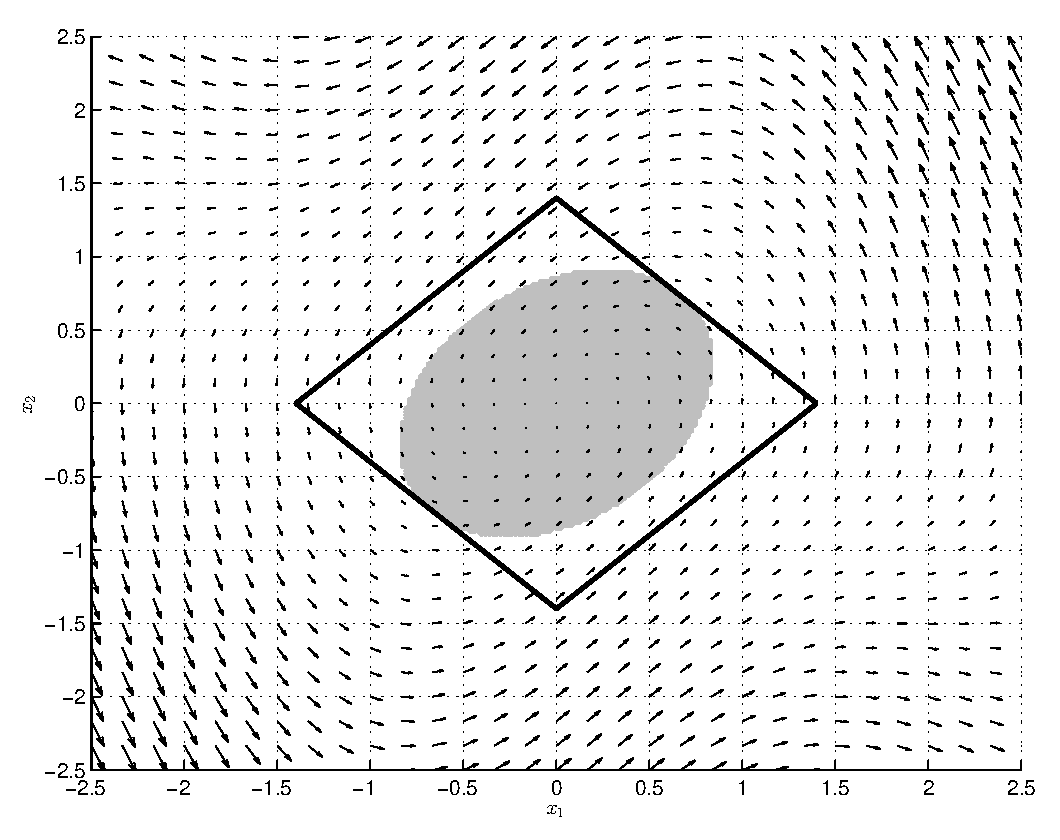
\includegraphics[width=0.95\linewidth]{exemplo2_13.eps}
  \caption{Estimativa da Região de Atração da Origem para o Exemplo 2.}
  \label{fig:rao2}
\end{figure}

\section{Conclusão}
O método proposto mostra-se efetivo e, através do pacote YALMIP \cite{proceedings:Lofberg2004}, de simples implementação.
Além disso, a formulação do problema por LMIs permite agregar eventuais restrições adicionais.
Finalmente, cabe destacar que diferentes escolhas, como o formato do politopo e o critério de otimização, influenciam diretamente na estimativa obtida para a região de atração.

\bibliographystyle{IEEEtran}
\bibliography{articles,books,proceedingsIEEE,controlIEEE}

\end{document}
